\chapter{Входные и выходные данные}

Входные данные: базовый $URL$---адрес веб-сайта, с которого будут загружаться страницы; режим работы --- последовательный или параллельный; количество страниц для загрузки в последовательном режиме или количество потоков (от 1 до 16) в параллельном режиме.

Выходные данные: файлы, каждый из которых содержит ссылки на рецепты блюд конкретной страницы с указанного веб-сайта.

\chapter{Преобразование данных}

В интерфейсе программы выбирается один из двух режимов: последовательный или параллельный. По нажатии кнопки <<Начать парсинг>> программа считывает базовый $URL$---адрес, а также количество страниц или количество потоков, в зависимости от выбранного режима, из полей ввода. Программа загружает $HTML$---контент страниц с указанного веб-сайта, а затем сохраняет загруженные страницы в соответствующую директорию ($seqfiles$ для последовательного режима и $parfiles$ для параллельного). Также программа выводит в консоль сообщения о ходе выполнения и возможных ошибках.

\chapter{Пример работы программы}

На рисунках \ref{fig:1-prog} --- \ref{fig:2-prog} представлен пример работы программы в последовательном режиме. В данном случае программа последовательно обрабатывает $4$ страницы сайта $https://food.ru/recipes/zakuski$; с каждой страницы программа сохраняет ссылки на рецепты в отдельный файл в директорию $seqfiles$. Содержимое одного из файлов представлено на рисунке \ref{fig:5-out}. Сообщения, связанные с парсингом, программа выводит в консоль.

\clearpage

\begin{figure}[]
	\centering
	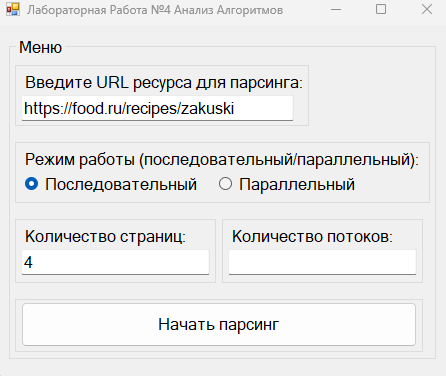
\includegraphics[scale=0.8]{img/1-prog.png}
	\caption{Ввод данных в интерфейс приложения}
	\label{fig:1-prog}
\end{figure}
\begin{figure}[]
	\centering
	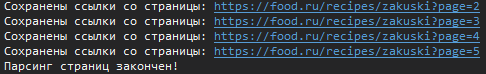
\includegraphics[scale=0.8]{img/2-prog.png}
	\caption{Сообщения о ходе выполнения парсинга}
	\label{fig:2-prog}
\end{figure}

\begin{figure}[]
	\centering
	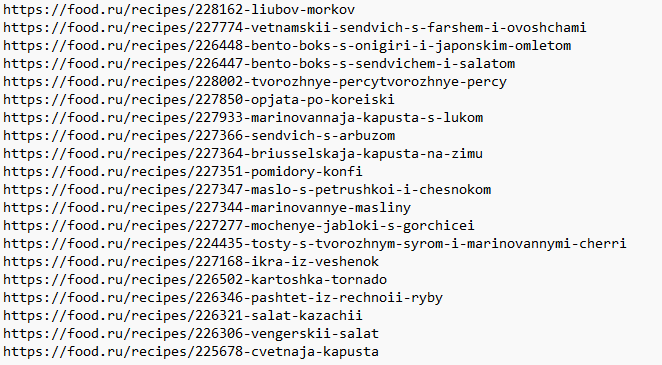
\includegraphics[scale=0.8]{img/5-outputfile.png}
	\caption{Содержимое выходного файла}
	\label{fig:5-out}
\end{figure}

На рисунках \ref{fig:3-prog} --- \ref{fig:4-prog} представлен пример работы программы в параллельном режиме. В данном случае программа создает для обработки каждой страницы свой отдельный поток. После создания всех потоков и выдачи им задач главный поток блокируется на время парсинга всех страниц. Каждый поток сохраняет ссылки на рецепты в отдельный файл в директорию $parfiles$. Сообщения, связанные с парсингом, каждый поток выводит в консоль по принципу взаимоисключения [2], так как консоль в данном случае является разделяемым ресурсом.

\begin{figure}[]
	\centering
	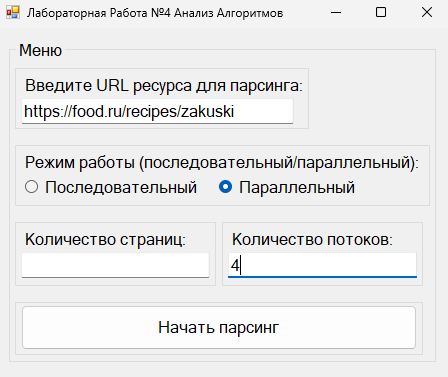
\includegraphics[scale=0.8]{img/3-prog.png}
	\caption{Ввод данных в интерфейс приложения}
	\label{fig:3-prog}
\end{figure}
\begin{figure}[]
	\centering
	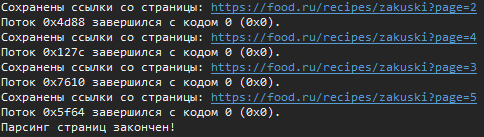
\includegraphics[scale=0.8]{img/4-prog.png}
	\caption{Сообщения о ходе выполнения парсинга}
	\label{fig:4-prog}
\end{figure}

\clearpage

\chapter{Тестирование}

Выполнено тестирование реализованной программы по методологии черного ящика. В таблице \ref{tbl:func} представлено описание тестов. Все тесты пройдены успешно.

\begin{table}[h!]
    \begin{center}
		\begin{threeparttable}
    \caption{Описание тестовых случаев}
    \captionsetup{justification=raggedright, singlelinecheck=false}
    \label{tbl:func}
    \begin{tabular}{|c|p{6cm}|p{6cm}|c|}
        \hline
        \textbf{№} & \textbf{Входные данные} & \textbf{Ожидаемый результат} & \textbf{Результат теста} \\
        \hline
        1 & Корректный базовый URL, последовательный режим, 5 страниц & Успешная загрузка 5 страниц, сохранение в \texttt{seqfiles} & Пройден \\
        \hline
        2 & Пустой базовый URL & Вывод сообщения об ошибке, запрос корректного URL & Пройден \\
        \hline
        3 & Некорректный базовый URL (без протокола) & Вывод сообщения об ошибке, запрос корректного URL & Пройден \\
        \hline
        4 & Корректный базовый URL, параллельный режим, 4 потока & Успешная загрузка страниц, сохранение в \texttt{parfiles} & Пройден \\
        \hline
        5 & Корректный базовый URL, параллельный режим, 20 потоков (превышение допустимого числа) & Вывод сообщения об ошибке, запрос корректного числа потоков (1-16) & Пройден \\
        \hline
        6 & Отключенное интернет-соединение & Вывод сообщений об ошибках при загрузке страниц & Пройден \\
        \hline
        7 & Корректный URL, последовательный режим, 0 страниц & Вывод сообщения об ошибке, запрос корректного числа страниц & Пройден \\
        \hline
        8 & Корректный URL, параллельный режим, отрицательное число потоков & Вывод сообщения об ошибке, запрос корректного числа потоков & Пройден \\
        \hline
    \end{tabular}
    \end{threeparttable}
    \end{center}
\end{table}

\clearpage

\chapter{Описание исследования}

Зависимости времени обработки страниц от количества страниц для последовательного и параллельного алгоритма (с 16 потоками) представлены на рисунке \ref{fig:tm}. Зависимости времени обработки страниц от количества страниц для последовательного и параллельного алгоритма (с 10000 потоками) представлены на рисунке \ref{fig:tm2}.
\begin{figure}[h]
    \centering
    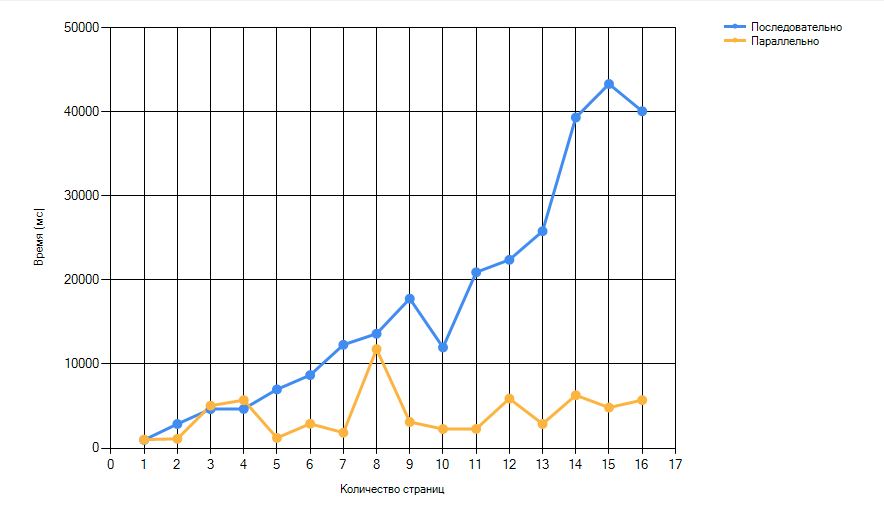
\includegraphics[width=0.7\linewidth]{img/6-research.png}
    \caption{Сравнение алгоритмов по времени}
    \label{fig:tm}
\end{figure}
\begin{figure}[h]
    \centering
    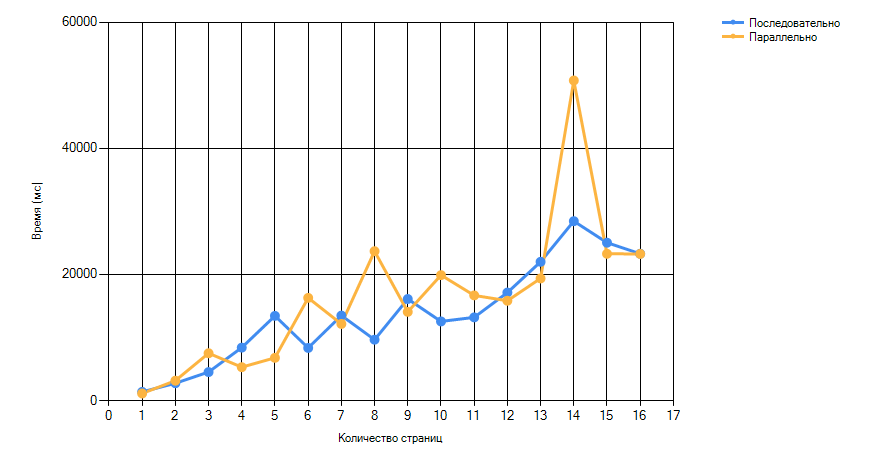
\includegraphics[width=0.7\linewidth]{img/7-research.png}
    \caption{Сравнение алгоритмов по времени}
    \label{fig:tm2}
\end{figure}

\clearpage
В результате исследования было получено, что параллельный алгоритм, использующий 16 нативных потоков, работает быстрее последовательного при количестве страниц большим или равном $5$. При обработки 16 страниц параллельный алгоритм работает почти в 8 раз быстрее последовательного. Однако параллельный алгоритм, использующий 10000 нативных потоков, работает при некотором количестве страниц медленнее последовательного. Так как операционная система вынуждена затрачивать ресурсы на поддержку большого количества потоков, то общее время выполнения алгоритма увеличилось. 
% \clearpage


